% Prof. Dr. Ausberto S. Castro Vera
% UENF - CCT - LCMAT - Curso de Ci\^{e}ncia da Computa\c{c}\~{a}o
% Campos, RJ,  2021
% Disciplina: Paradigmas de Linguagens de Programa\c{c}\~{a}o
%


\chapter{Aplicações da linguagem}

Neste capítulo vamos apresentar cinco exemplos de aplicações escritas na linguagem Julia, bem como seus respectivos códigos-fonte, e imagens demonstrando seu funcionamento. 

\section{Quicksort}
A ordenação de elementos em listas ou vetores é uma das operações computacionais mais importantes. 

Desse modo apresentamos o Quicksort, dos principais algoritmos de ordenação, sendo, inclusive, utilizado por padrão na função de ordenação (\href{https://github.com/JuliaLang/julia/blob/2364748377f2a79c0485fdd5155ec2116c9f0d37/base/sort.jl#L259-L296}{sort!()}) nativa da linguagem. 
\newline

Esse algoritmo se inicia elencando um elemento no vetor para ser o pivô dessa execução. 
A partir de então todos os elementos menores ou iguais ao pivô são colocados antes do mesmo e consequentemente todos os elementos maiores são colocados nas posições seguintes ao pivô. 

Em seguida é feito uma chamada recursiva da mesma função para cada uma dessas duas porções -do primeiro elemento até o anterior ao pivô, e do elemento seguinte ao pivô até o último. 

No Código \ref{quicksort_code}, apresentamos uma implementação do algoritmo disponível na wiki \href{https://rosettacode.org/wiki/Sorting_algorithms/Quicksort#Julia}{Rosetta Code}. 
Nela, o mecanismo principal de pivotagem se por meio de duas variáveis que guardam o último elemento da porção inferior ao pivo (left) e o primeiro elemento da porção superior ao pivô (right). Ou seja, os limites internos, visto que os limites externos serão os próprios primeiro e último elementos do vetor. 

Desse modo, essas variáveis dos limites internos se iniciam iguais aos limites externos, se aproximando do pivô da seguinte forma: 
caso o atual índice left seja menor que o pivo, o índice se desloca mais um elemento a direita.
Caso o atual índice right seja maior que o pivô ele se desloca para a esquerda.
Ambas ocorrem até que cheguem em um elemento fora de lugar, nesse caso o elemento fora de lugar em cada porção são permutados. 
Assim, temos duas porções para abrigarem os elementos maiores e menores que o pivô, que se iniciam vazias, mas vão avançando em direção ao pivô até que englobem todos os elementos. 

Na Fig.\ref{quicksort} implementamos o código no ambiente integrado de desenvolvimento (IDE) \href{https://code.visualstudio.com/docs}{Visual Studio Code} e demonstramos seu funcionamento com um vetor exemplo. 

[TODO: modificar o termo "listing" para algum outro?] 
\begin{lstlisting}[label={quicksort_code},caption={Implementação do algoritmo quicksort em Julia}]
  function quicksort!(A,i=1,j=length(A))
  if j > i
      pivot = A[rand(i:j)] 
      left, right = i, j
      while left <= right
          while A[left] < pivot
              left += 1
          end
          while A[right] > pivot
              right -= 1
          end
          if left <= right
              A[left], A[right] = A[right], A[left]
              left += 1
              right -= 1
          end
      end
      quicksort!(A,i,right)
      quicksort!(A,left,j)
  end
  return A
end
\end{lstlisting}

\begin{figure}[H]
   \begin{center}
       \caption{Quicksort na IDE VScode} \label{quicksort}
       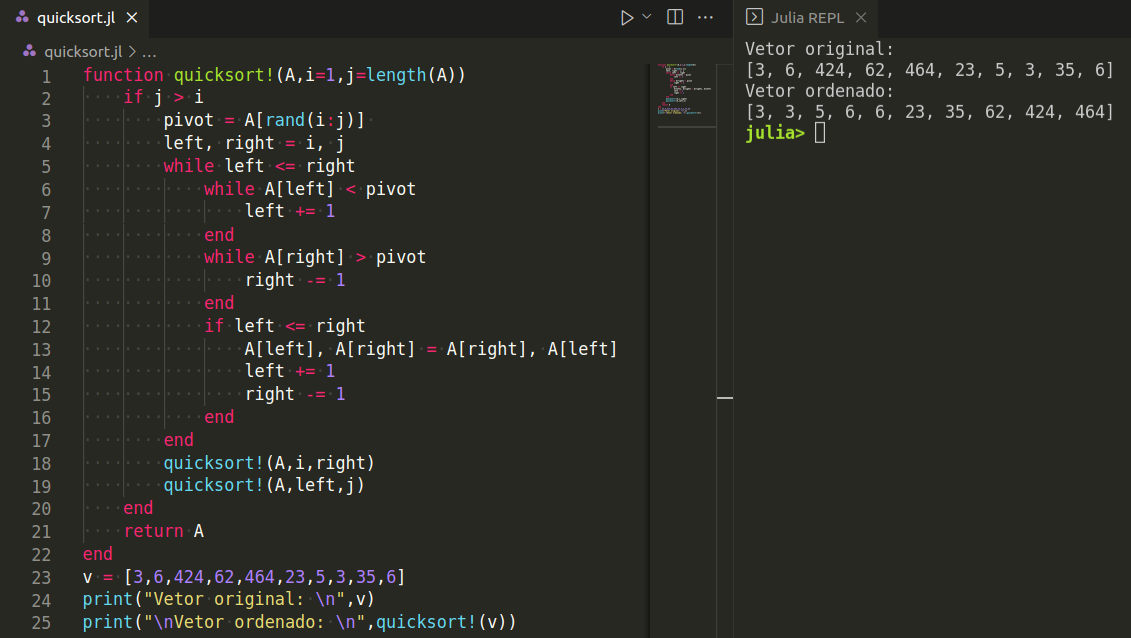
\includegraphics[width=12cm]{aplicacoes/quicksort.png} \\
       {\tiny \sf Fonte: Autor}
   \end{center}
\end{figure}

\section{Calculadora}
Outro aspecto muito importante da computação envolve o uso de interfaces gráficas para facilitar a interação do usuário com a máquina.
%, tanto no quesito acessibilidade quanto na acessibilidade de . 
Entretanto a construção de janelas, botões e afins é uma tarefa complexa, de modo que na maior parte dos casos os programadores utilizam uma biblioteca que implementa tais componentes de interface gráfica, sendo as duas mais famosas a Qt e a GTK chamadas de GUI Toolkit. %TODO refatorar esse parágrafo

Nesse exemplo demonstramos uma calculadora simples utilizando a biblioteca Gtk.jl que traz a bilbioteca GTK de forma amigável para a linguagem Julia. 

O código \ref{calculadora_code} apresenta de modo compacto a implementação criada por Nand Vincchi está está disponível como exemplo no repositório \href{https://github.com/JuliaGraphics/Gtk.jl/blob/master/example/calculator.jl}{Github} da biblioteca Gtk.jl. 

Adicionamos as linhas para instalar o pacote Gtk, caso o mesmo ainda não esteja presente. O código original segue importando o pacote, e criando uma janela com título "Calculator", cria-se todos os botões, seguido de 4 chamadas "caixas" horizontais que são preenchidas com os botões criados. Cria-se uma caixa vertical para receber as quatro horizontais, a "tela" da calculadora, e espaços. Por sua vez essa caixa vertical é adicionada a janela.

Finalmente temos a função \_button\_clicked\_callback que adiciona responsividade dos botões de compor uma string que é apresentada na tela conforme são apertados, e ao clicar no igual a string contruída é enviada a função "calculate" que a processa e retorna o resultado que será apresentado na tela.

Na figura \ref{calculadora} podemos ver a janela gráfica e parte do código sendo executado na IDE. 

\begin{lstlisting}[label={calculadora_code},caption={Calculadora simples em GTK}]
# Simple calculator application that utilises Gtk.jl
# created by Nand Vinchhi for GCI 2019

using Gtk

win = GtkWindow("Calculator")

b1 = GtkButton("1")
b2 = GtkButton("2")
b3 = GtkButton("3")
b_plus = GtkButton("+")
[...]
 
hbox1 = GtkButtonBox(:h)
hbox2 = GtkButtonBox(:h)
hbox3 = GtkButtonBox(:h)
hbox4 = GtkButtonBox(:h)

push!(hbox1, b1)
push!(hbox1, b2)
push!(hbox1, b3)
push!(hbox1, b_plus)
[...]

vbox = GtkBox(:v)
label = GtkLabel("")
GAccessor.text(label,"")

push!(vbox, GtkLabel(""))
push!(vbox, label)
push!(vbox, GtkLabel(""))
push!(vbox, hbox1)
push!(vbox, hbox2)
push!(vbox, hbox3)
push!(vbox, hbox4)
push!(win, vbox)

text = ""

function calculate(s)
	x = "+ " * s
	k = split(x)
	final = 0
	
	for i = 1:length(k)
		
		if k[i] == "+"
			final += parse(Float64, k[i + 1])
		elseif k[i] == "-"
			final -= parse(Float64, k[i + 1])
		elseif k[i] == "x"
			final *= parse(Float64, k[i + 1])
		elseif k[i] == "/"
			final /= parse(Float64, k[i + 1])
		end
	end
	return string(final)
end

function button_clicked_callback(widget)
	if widget == b1
		global text = text * "1"
        GAccessor.text(label, text)
    elseif widget == b2
    	global text = text * "2"
        GAccessor.text(label, text)
    elseif widget == b3
    [...]
        elseif widget == b_equalto
    	global text = calculate(text)
        GAccessor.text(label, text)
    end
end

id1 = signal_connect(button_clicked_callback, b1, "clicked")
id2 = signal_connect(button_clicked_callback, b2, "clicked")
id3 = signal_connect(button_clicked_callback, b3, "clicked")
[...]

showall(win)

\end{lstlisting}


\begin{figure}[H]
   \begin{center}
       \caption{Janela GTK da calculadora e vscode} \label{calculadora}
       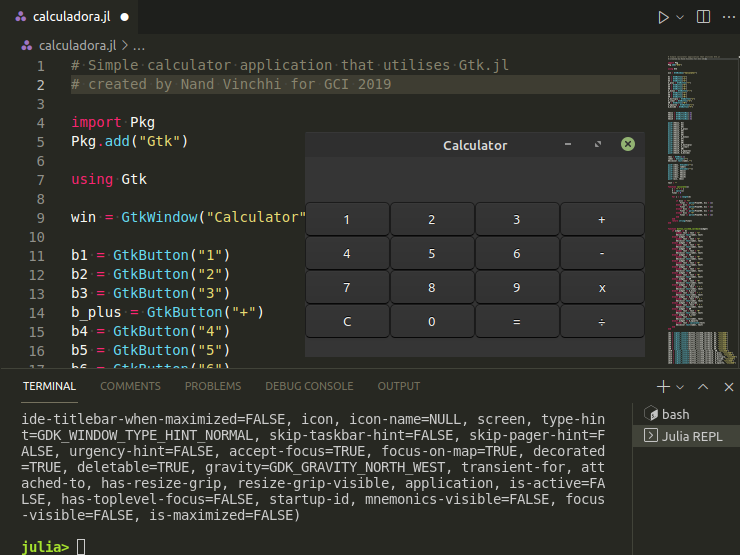
\includegraphics[width=12cm]{aplicacoes/calculadora.png} \\
       {\tiny \sf Fonte: Autor}
   \end{center}
  \end{figure}






\section{Plotagem (Iris data set)}
Igualmente importante no ecossistema Julia é a habilidade de analisar dados. Nesse exemplo demonstramos as funções básicas para ler um arquivo csv, utilizar um DataFrame, e plotar um gráfico que permita análisar esse dados. 

Para tanto, utilizamos o famoso Iris-dataset \cite{Fisher1936}, onipresente na literatura estatística e muito utilizado justamente para demonstrar um ecossistema de análise de dados. 

Esse dataset consiste na observação de 50 exemplares de três epecécies de flores do gênero Iris (Fig. \ref{iris_flowers}), para cada observação temos o comprimento e largura de suas sépalas e pétalas bem como a qual espécie tais medidas pertecem (Fig.\ref{iris_data}).

\begin{figure}[H]
   \begin{center}
       \caption{Flores do gênero iris} \label{iris_flowers}
       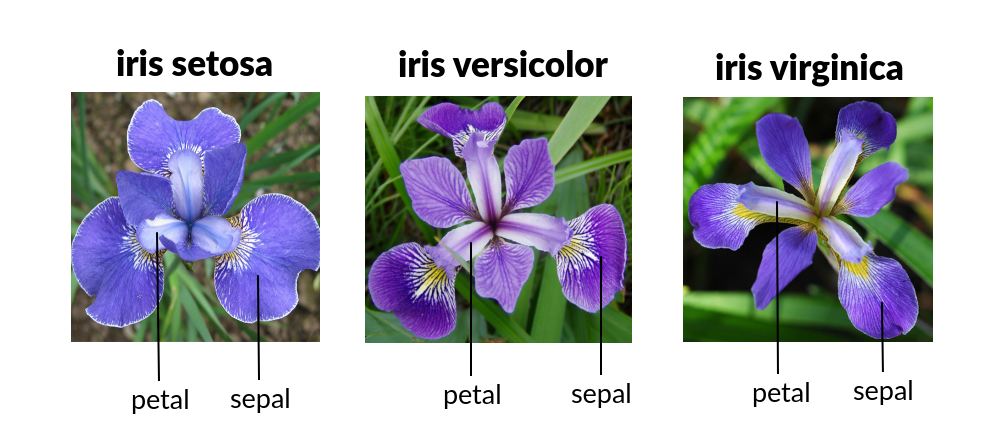
\includegraphics[width=12cm]{aplicacoes/iris-flowers.png} \\
       {\tiny \sf Fonte: https://rpubs.com/mbatista/545937}
   \end{center}
\end{figure}

\begin{figure}[H]
   \begin{center}
       \caption{Iris Dataset} \label{iris_data}
       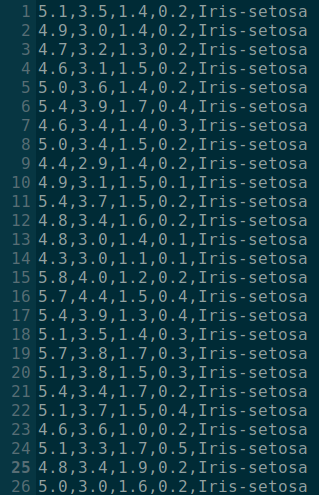
\includegraphics[width=5cm]{aplicacoes/iris_data.png} \\
       {\tiny \sf Fonte: https://archive.ics.uci.edu/ml/datasets/Iris/https://archive-beta.ics.uci.edu/ml/datasets/iris}
   \end{center}
\end{figure}

Assim, utilizamos o ambiente de desenvolvimento \href{https://jupyter.org/}{Jupyter Notebook}, que consiste em cadernos compostos por células interativas. 
Na figura \ref{iris_pacotes} temos a instalação dos pacotes: CSV para a leitura do arquivo com os dados, DataFrame que é a estrutura de dados padrão em tabelas, e DataVoyager que apresenta uma interface simples e interativa para plotagem exploratória de gráficos.

\begin{figure}[H]
   \begin{center}
       \caption{Instalação das bibliotecas} \label{iris_pacotes}
       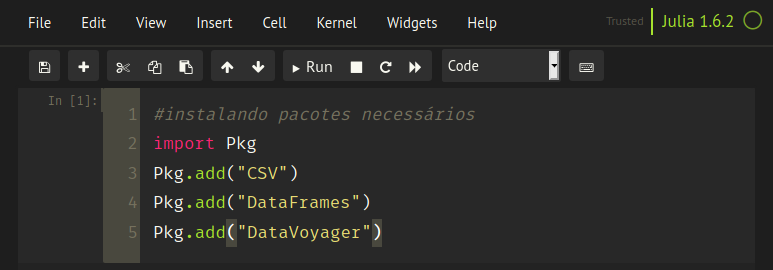
\includegraphics[width=12cm]{aplicacoes/iris_pacotes.png} \\
       {\tiny \sf Fonte: Autor}
   \end{center}
\end{figure}

Na figura \ref{iris_csv} importamos as bibliotecas CSV e DataFrames, criamos uma variável com o cabeçalho das colunas e finalmente lemos o arquivo csv e o armazenamos em memória na variável "iris". No retorno podemos ver parte do dataframe.

\begin{figure}[H]
   \begin{center}
       \caption{Leitura do CSV} \label{iris_csv}
       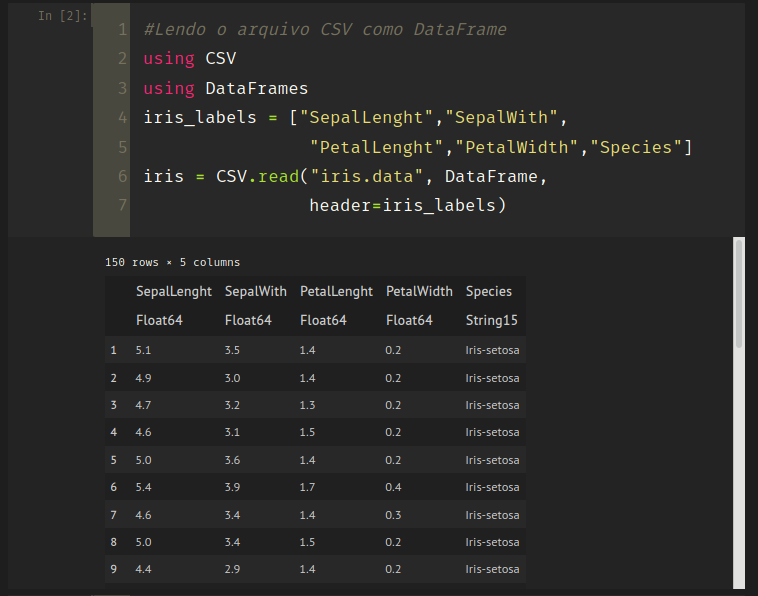
\includegraphics[width=12cm]{aplicacoes/iris_CSV.png} \\
       {\tiny \sf Fonte: Autor}
   \end{center}
\end{figure}

Já na figura \ref{iris_plot} temos a interface do DataVoyager, onde selecionamos o comprimento e largura das pétalas para os eixos bem como que a cor de cada ponto se dá de acordo com a espécie relacionada aquele ponto. O programa automaticamente nos retorna um scatter plot, conforme nossas especificações, e ainda sugere outras abordagens. 


\begin{figure}[H]
   \begin{center}
       \caption{Plotagem com DataVoyager} \label{iris_plot}
       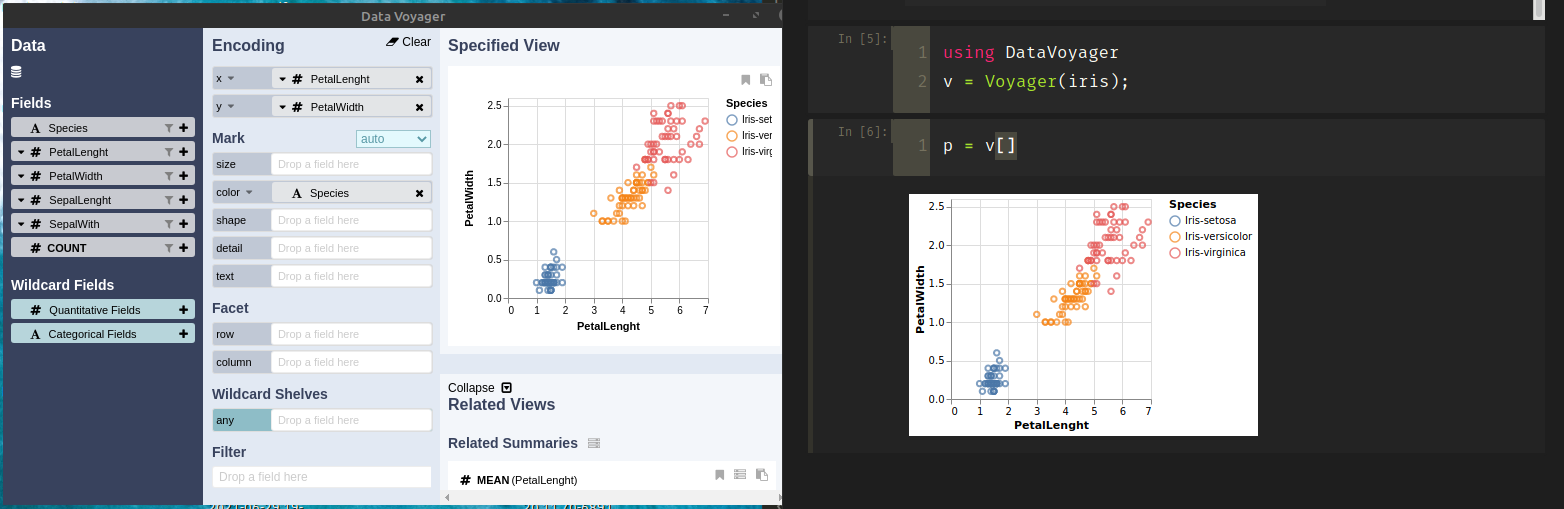
\includegraphics[width=15cm]{aplicacoes/iris_plot.png} \\
       {\tiny \sf Fonte: Autor}
   \end{center}
\end{figure}

Assim, torna-se evidente o potencial da linguagem e suas ferramentas para a análise exploratória de dados e construção de vizualizações. 

%\subsection{texto removido da seção principal}
%em dados esse é o equivalente ao "hello, world!", o conjunto de dados das dimensões espaciais de três especies de flores coletada por ninguém menos que R.A Fisher, um dos pais da estatística. A ideia é que a facilidade de se trabalhar com esse conjunto de dados nos permite conhecer o ecossistema de dados de uma linguagem. 

%Desse modo, intalamos os pacotes necessários (Fig TAL), isto é, CSV para ler o arquivo, DataFrames para utilizarmos essa estrutura de dados, e o DataVoyager para explorar os dados e construir interativamente uma plotagem que nós permita compreender a relação entre as métricas e suas respectivas espécies. 

%Para tanto, baixamos o \href{https://archive.ics.uci.edu/ml/datasets/Iris/https://archive-beta.ics.uci.edu/ml/datasets/iris}{dataset}, utilizamos a biblioteca CSV para ler o arquivo e salva-lo como DataFrame na memória, em seguida utilizamos a biblioteca Plots para graficar os dados das flores.
% de modo a permitir futuras abordagens na busca matematicamente classificar uma dessas flores partindo apenas das dimensões de suas pétalas e sépalas. 
%"hello, world!" da programação, 
%Igualmente importante é a capacidade plotar gráficos, nesse exemplo nos usamos a função nativa de ler arquivos CSV 

%É possível classificar uma dessas flores tão parecidas apenas a partir das dimensões de altura e largura de suas sepas e petálas. 

\section{Banco de Dados SQL lite}
Outro aspecto fundamental de uma linguagem é a sua integração com banco de dados. Aqui trazemos um exemplo simples da criação e uso de um banco de dados SQLite, por meio da sua biblioteca disponível em Julia. 

Após intalarmos o pacote SQLite.jl, criamos um objeto e arquivo de banco de dados. Em seguida construímos uma função que lê o input padrão do teclado, separa a frase do autor e armazena ambos no banco de dados criado, conforme demostra e explica a figura \ref{sql_corpo}.
Esse código foi inspirado no seguinte exemplo disponível no Github. \footnote{https://github.com/julia4ta/tutorials/blob/master/Series\%2004/Tutorial\%2004x05/sourcecode.jl}


%\begin{figure}[H]
%   \begin{center}
%       \caption{Instalação do pacote SQLite.jl} %\label{sql_pacote}
%       \includegraphics[width=12cm]{aplicacoes/%sql_pacote.png} \\
%       {\tiny \sf Fonte: Autor}
%   \end{center}
%\end{figure}
%
\begin{figure}[H]
   \begin{center}
       \caption{Corpo do programa que armazena as frases} \label{sql_corpo}
       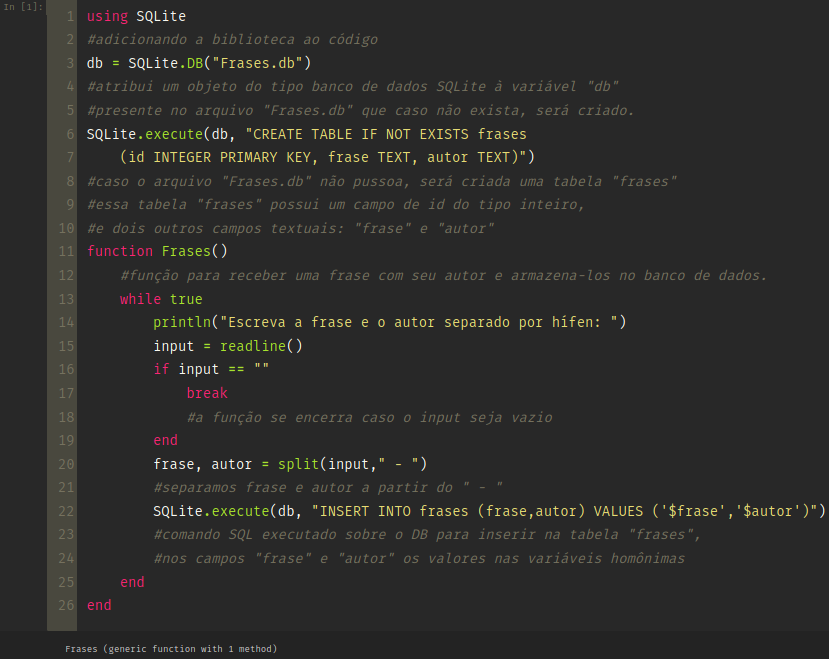
\includegraphics[width=12cm]{aplicacoes/sql_corpo.png} \\
       {\tiny \sf Fonte: Autor}
   \end{center}
\end{figure}
Em seguida executamos a função "Frases()" escrevendo três entradas de frases com seus respectivos autores conforme a figura \ref{sql_frases}. 
\begin{figure}[H]
    \begin{center}
        \caption{Função "Frases()" sendo executada} \label{sql_frases}
        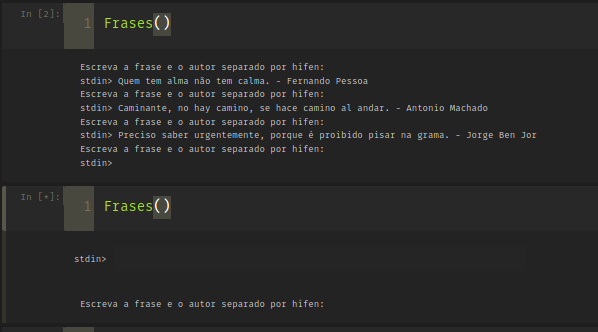
\includegraphics[width=12cm]{aplicacoes/sql_frases.png} \\
        {\tiny \sf Fonte: Autor}
    \end{center}
\end{figure}
Finalmente, na figura \ref{sql_query}, efetuamos uma busca SQL nesse banco de dados. Selecionamos todos os campos da tabela frases, e como não utilizamos o WHERE para restringir determinadas entradas, essa query retorna todo o conteúdo da tabela frases. 
Interessante notar que o comando SQLite.DBInterface.execute() retorna um objeto, que transformamos em DataFrame para o acessarmos. 

\begin{figure}[H]
   \begin{center}
       \caption{Query do banco de frases criado} \label{sql_query}
       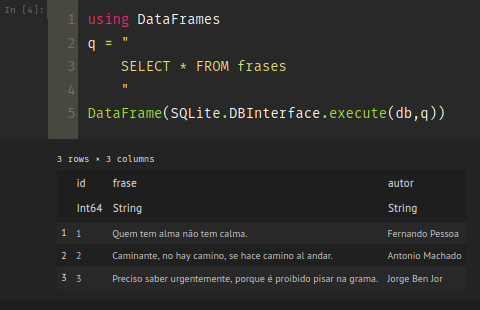
\includegraphics[width=12cm]{aplicacoes/sql_query.png} \\
       {\tiny \sf Fonte: Autor}
   \end{center}
\end{figure}
%Aqui trazemos dois exemplos de utilização do banco de dados SQLite. No primeiro nós criamos um arquivo de banco de dados, preenchemos com algumas informações e as recuperamos. Já no segundo demonstramos uma query no famoso banco de dados \href{https://github.com/lerocha/chinook-database/blob/master/ChinookDatabase/DataSources/Chinook_Sqlite.sqlite}{Chinook}, que seria em SQL o equivalente ao Iris Dataset em Data Analysis. 
%#A princípio vou deixar só o meu primeiro exemplo mesmo, pra não ter que explicar sobre o chinook e tal








%\section{Pesquisa operacional}
%Nesse exemplo utilizamos a biblioteca JuMP.jl que nos dá uma interface unificada para utilizar diversos motores de resolução de problemas lineares.



%Dataframes em julia?
%Matrizes em Julia? Linear solver? 
%Operational research? 
%Data Wrangling?
%Pesquisar nos videos do Grant 3b1b e no 



